\chapter{IDL}

\section{Définition du langage IDL:}

IDL ou \textbf{L}angage de \textbf{D}onnées \textbf{I}nteractif est un langage de programmation utilisé pour créer des applications effectuant une analyse de données, il est principalement utilisé par les astronomes et les experts en imagerie médicale ou le traitement d'image numérique nécessite une vitesse élevée dans de nombreuses applications.\\
Il est issu du logiciel interactif de traitement de données solaires ANA conçu par le groupe de physique solaire de la NASA au début des années 1980 pour le traitement des données du satellite Solar Maximum Mission. Aujourd'hui IDL s'est imposé comme LE système de traitement universel utilisé en physique solaire, et son succés débord désormais vers tous les horizons astronomiques.

 \section{une procédure IDL:}
 Un programme IDL se rédige à l’intérieur d'un éditeur de texte indépendant selon:\\
Pro nom\_programme\\
   Suite d’Instructions\\
end\\
Si ce fichier programme porte le nom nom\_programme.pro on le compile en tapant sur
le prompt IDL la commande suivante:\\
IDL> .run nom\_programme\\
puis on l’exécute en appelant le programme directement par son nom :\\
IDL> nom\_programme\\
On peut passer des variables à une procédure en entrée sortie. Par exemple avec var\_in
en entrée et var\_out en sortie:\\
Pro nom\_programme, var\_in, var\_out\\
  Suite d’Instructions\\
End\\
puis on exécute la procédure en appelant le programme directement par son nom :\\
IDL> nom\_programme, var\_in, var\_out


\section{Structure syntaxique d'un module IDL:}

<module> /* un contexte ou espace de nommage */\\

<déclaration de types>\\
<déclaration de constantes>\\
<déclaration d'exceptions>\\

interface /* une classe */\\
<déclaration de types>\\
<déclaration de constantes>\\
<déclaration d'exceptions>\\

<déclaration d'attributs> /* variables */\\
<déclaration d'opérations> /* méthodes */\\
<modules>\\


\section{Les variables dans IDL:}
IDL travaille avec des variables de tout type :
\begin{itemize}[label=$\bullet$]
\item Octets 8 bits de 0 à 255 (type BYTE)
\item Entiers courts 16 bits signés de –32768 à 32767 (type FIX ou INT)
\item Entiers courts 16 bits non signés de 0 à 65535 (type UINT)
\item Entiers longs 32 bits signés (type LONG)
\item Entiers longs 32 bits non signés (type ULONG)
\item Réelles 32 bits dits simple précision (type FLOAT), 7 chiffres significatifs entre ±1038
\item Réelles 64 bits dites en double précision (type DOUBLE), 14 chiffres significatifs
\item Complexes 64 bits (type COMPLEX), 7 chiffres significatifs entre ±1038
\item Complexes 128 bits (type DCOMPLEX), 14 chiffres significatifs entre ±10308
\item Chaînes de caractères (type STRING)
\end{itemize}

\section{Le contrat IDL:}
Il permet d'exprimer, sous la forme d'un contrat, la coopération entre les fournisseurs et les utilisateurs de services. Il sépare l'interface des objets de leur implantation et masque les problèmes liés à la localisation des objets, à l'interopérabilité et à l'hétérogénéité. Il spécifie sous la forme d'interfaces IDL les types manipulés par un ensemble d'applications réparties.\\
Le contrat IDL rend transparent aux fournisseurs et clients l'infrastructure logicielle et matérielle. Il met client et fournisseur en relation à travers un bus CORBA.\\
La compilation d'un contrat IDL créé une souche (talon) IDL (ou SII, interface d'invocation statique) dans l'environnement de programmation du client et une souche (squelette) IDL (ou SSI, interface de squelette statique) dans l'environnement de programmation du fournisseur.
Le client invoque localement la souche pour accéder à l'objet. La souche construit alors la requête qui est ensuite transportée par le bus logiciel pour être délivrée au squelette IDL (coté serveur donc) qui la délègue à l'objet.\\

\section{Mappings:}
Un mapping est une traduction des éléments fournis par l'IDL en éléments d'un langage de programmation.\\
Les principaux mappings disponibles sont : C, C++, Java, Smalltalk, CLOS, Python, Ada95, Cobol Objet.\\
Les compilateurs IDL ne traduisent que des squelettes. Les objets clients utilisent ces squelettes pour déterminer les opérations légales qu'ils peuvent invoquer sur un serveur. Les objets serveur fournissent une implantation pour ces squelettes.

\section{Référentiel d'interfaces:}
C'est une base de données en ligne de définitions d'objets, d'interfaces, de modules. Les définitions d'objets sont fournies par les compilateurs d'IDL ou par des fonctions d'écriture du référentiel.
Les référentiels d'interfaces peuvent se fédérer et coopérer à travers les ORBs.

\vspace*{2cm}

\begin{figure}[h]
        \centering
     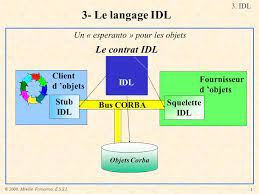
\includegraphics[scale= 1]{IDL/3}
        \caption{IDL}
\end{figure}

\pagebreak
\vspace*{9cm}
\begin{center}
   \Huge{** FIN **}
\end{center}